\documentclass[10 pt, technote]{IEEEtran}

\usepackage{multicol}
\usepackage{lipsum}
\usepackage{graphicx}
\usepackage{float}

\title{When N-Detect Doesn't Detect: Cell-Aware-Type Faults and Stuck-At ATPG}
\author{Fanchen~Zhang, Micah~Thornton, Jennifer~Dworak}
\begin{document}
\twocolumn[
  \begin{@twocolumnfalse}
    \maketitle
  \end{@twocolumnfalse}
]

\begin{abstract}

Cell-aware faults have been proposed to more effectively detect defects within gates.  We investigate the effectiveness of different types of ATPG for efficiently detecting cell-aware-type faults that are most important during functional operation.

\end{abstract}

\tableofcontents

\section{Introduction}

\section{Previous Work}

%	Chip design manufacturers have always needed ways to speed up the testing process in order to push out their products more quickly. As a side effect of that, there has been much work done on n-detect, cell-aware, and stuck-at testing as these methods have been shown to significantly speed up the process. The optimization of test sets has been a long sought after goal one method of achieving this optimization is fault criticality as discussed by Shi et al~\cite{4641197}~\cite{5469545}.In their paper on fault models, Hapke, and Schloeffel introduced the method of cell-aware test pattern generation~\cite{6233046}. Similarly, in their paper: Rajski et al examined the usefulness of the cell-aware model in improving tests as well as maintaining the efficiency of previous models (as related to 20 nm technologies)~\cite{6673230}. Again in later research Hapke, this time collaborating with Rajski et al examined the results of their use of cell aware test pattern generation in order to test 1\,900 different cells in 800\,000, 32 nm components, and determined that defect-rate was reduced overall~\cite{6401533}. Hapke et al again proved the usefulness of the new cell aware fault modeling system when they tested 1\,500 CMOS 65 nm cells that were being used in automobiles~\cite{5783604}. In yet another earlier paper Hapke et al compared the new cell aware approach to previous approaches such as: ``gate-exhaustive, n-detect, or embedded multi-test"~\cite{5355741}. In our research we also take these other methods into account, but also realize that we don't need to have a product which is 100\% defect free, and that we are really using the error tolerance model as described by Fang et al in relation to video compression hardware~\cite{6114751}. 
	
%N-Detect generally seems as though it decreases the defect rate in hardware while increasing the test set size, as shown by Huang~\cite{1613177} as well as McCluskey et al~\cite{894222}. Later Alves et al examined the implicit increase in size of the test set based on n-detect and proposed methods for decreasing the test set size~\cite{5361309}. 
%
%Our research inherently relies on being able to define our own fault model to use in test simulation. There are several ways to come up with your own fault model. We defined our model in a UDFM(User Defined Fault Model). This method relies on having what are called fault tuples as described by Dwarakanath~\cite{Dwarakanath:2000:UFS:337292.337779}.

	When a manufacturer goes about designing their test set, they have to realize that there is always an inherent trade off between the time used to complete the test and the coverage of defaults by the test set. Thus their goal is to examine a method whereby test pattern sets are created that are both effective and efficient. 
	
	In 1959 Eldred discovered a fault model called the ``stuck-at fault model" that has since been used to generate a highly effective test set of a reasonable size~\cite{Eldred:1959:TRB:320954.320957} This model, unfortunately, breaks down in the presence of faults that do not behave as stuck-at faults. For these faults variations of n-detect test sets(which require that each fault be detected $n$ times, where $n > 1$) are used. These tests obtain better fortuitous detection of faults that did not fit the model~\cite{529895}~\cite{766662}~\cite{923462}.
	
	The notion of these n-detect test sets have been extended and optimized even further to ensure that each additional detection provides the best possible value, including the maximum excitation balance~\cite{Dworak:2004:BEE:968879.969191}. Some have even considered the site values in a particular region around a particular gate~\cite{Dwarakanath:2000:UFS:337292.337779}. 
	
	Other researchers in addition have proposed gate exhaustive tests, which attempt to ensure that all possible input combinations for each gate are tested~\cite{894222}. These methods have a much higher defect coverage, but follow the general trade off between fault coverage and test time as discussed above. 
	
	All of the previously mentioned faults deal with the values that occur on the wires, and do not necessarily consider that faults can occur within the gates or ``cells" themselves. In order to address this variety of fault, the cell-aware fault model was presented~\cite{6233046}.This model was extensively tested and found to be a decent new model~\cite{6673230}~\cite{6401533}~\cite{5783604}. This model was subsequently compared with other models, and test set generation methods ~\cite{5355741}. The one unfortunate thing about considering these additional models, as expected, the more models tested for the greater the test duration. 
	
	Although certain models test for all the possible faults that fit a certain fault model, it might be more beneficial to only consider the faults that would significantly affect the end user of the product. In the past it has been shown that stuck-at faults can be graded based on fault criticality and how estimates of such can be used to create effective test sets when testing resources are limited ~\cite{5469545}~\cite{4641197}. Some researchers have even deemed that defective parts can be sold if it is unlikely that the end user will ever use the product in such a way that the defects that passed the test phase will ever effect them~\cite{Breuer:1985:KBS:317825.317868}~\cite{Hsieh:2007:RDA:1266366.1266717}. 
	
	
	
	  






\section{Algorithm/ Problem etc.}

\subsection{Cell-Aware Fault Models and their Relation to Stuck-at ATPG}

\subsubsection{Cell-aware fault detection conditions}

\subsubsection{Why n-detect ATPG Test Sets May Be Biased}

\subsection{Determining which Cell-aware faults to target}

\section{Experimental Setup \& Results}
\subsection{Set Up}
To approve the effectiveness of functional cell-aware detec-
tion, s38584, s38417, s15850, s13207 and s9234 are chosen
as benchmarks since they have more kind and larger number
of gates among ISCAS89.
The experiment Testing flow is shown in Fig.4. We create
two different Cell-Aware fault sets except for two inputs gates
as described in section 3. (Cell-Aware Fault Models and their
Relation to Stuck-at ATPG), replaced all primitive gates with
two more inputs by cell library. One Scan-Chain is inserted in
each benchmark for testing. Then ATPG testing pattern sets for
Stuck-at and Cell-aware faults are obtained on Mentor Graph-
ics Tessent. To achieve N-detect of Stuck-at model effects on
Cell-Aware faults, four setting up arguments for ATPG Stuck-
at are implemented; they are n0 (disable multiple detection
function), n1 (guaranteed detections=1, desired detections=3),
n2 (guaranteed detections=2, desired detections=5) and n3
(guaranteed detections=3, desired detections=7). According to
section 3, a test bench in which initializes DFFs as 0 to
engender DFFs into stable state is employed for capturing
Good-State sets when Synopsys VCS simulates a golden
benchmark. Note because the functionality of benchmarks are
unknown, random patterns are created to represent the real
functional inputs. In order to balancing randomness, we do
two times of creating random pattern sets for each number
of Good-States. Since UDFM of Tessent does not support
N detection, we split Good-state sets and APTG sets into
5 patterns per simulation pattern file and repeat simulation
processes multiple times.
\begin{figure}[htpb]
\centering
\textbf{Flow of Set Up} \\\hfill\\
\centerline{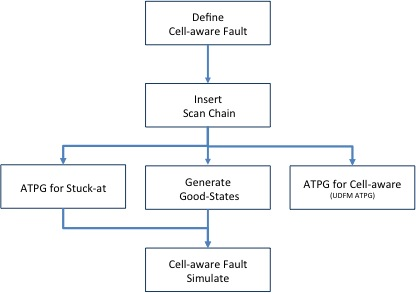
\includegraphics[scale=0.5]{Figures/experiment_flow.jpg}}
\end{figure}


\subsection{Results}

\begin{figure}[H]
\begin{center}
\textbf{Stuck-At Patterns V.S. Cell-Aware Top-Off Patterns}%\par\medskip
\end{center}
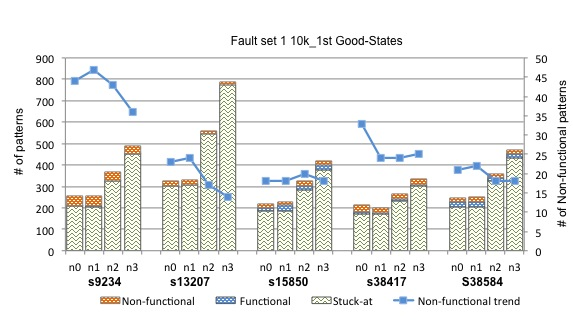
\includegraphics[scale=0.2,width = \linewidth]{../Figures/top_off_set1_10k_1st.jpg}
\end{figure}

\begin{figure}[H]
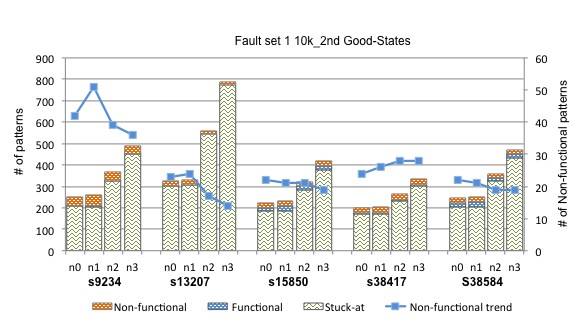
\includegraphics[scale=0.2,width = \linewidth]{../Figures/top_off_set1_10k_2nd.jpg}
\end{figure}

\begin{figure}[H]
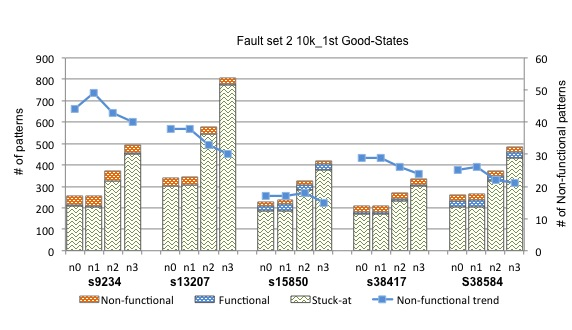
\includegraphics[scale=0.2,width = \linewidth]{../Figures/top_off_set2_10k_1st.jpg}
\end{figure}

\begin{figure}[H]
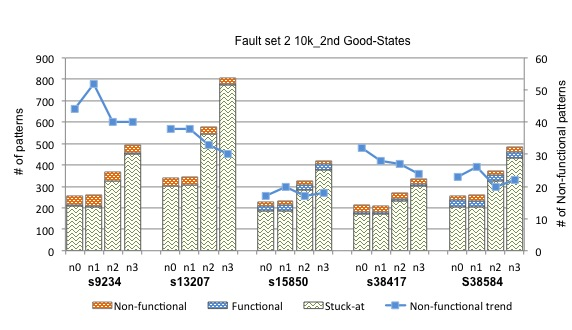
\includegraphics[scale=0.2,width = \linewidth]{../Figures/top_off_set2_10k_2nd.jpg}
\end{figure}

In the above figures we can see that two different generations of 10\,000 good-states used on two different permutations of Cell-aware fault set yielded similar results. Another observation is that in each of the four cases there are more patterns that test for non-functional defects than those that tests for functional defects that are generated by cell aware ATPG, even in comparison with the large number of patterns generated by stuck-at ATPG, the number of non-functional patterns is significant. The number of functional test patterns is negligible compared to the large amount of patterns generated by the stuck-at ATPG. Because adding all of the non-functional tests to the test set adds significant costs, these figures suggest that using n-detect with a higher degree of n can decrease the number of non-functional tests which will decrease the added costs associated with testing all of the non-functional defects. 

\begin{center}
\textbf{\% Increase in Test Length When Non-Functional Cell-Aware Faults are Included in the Fault Set}%\par\medskip
\end{center}
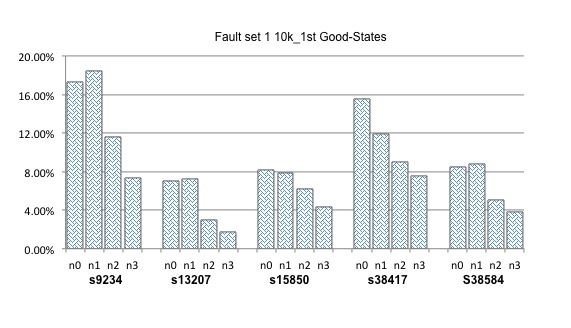
\includegraphics[scale=0.2,width = \linewidth]{../Figures/percentage_increase_set1_10k_1st.jpg}
\end{figure}

\begin{figure}[H]
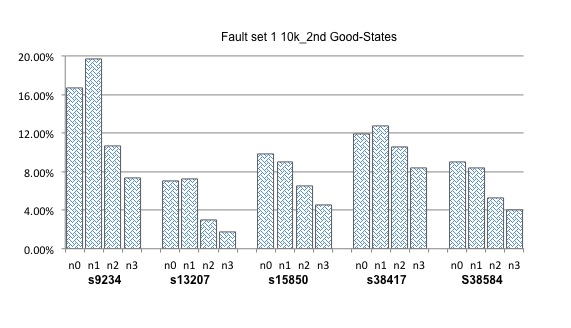
\includegraphics[scale=0.2,width = \linewidth]{../Figures/percentage_increase_set1_10k_2nd.jpg}
\end{figure}

\begin{figure}[H]
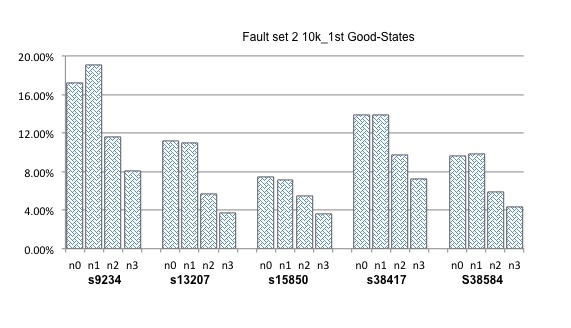
\includegraphics[scale=0.2,width = \linewidth]{../Figures/percentage_increase_set2_10k_1st.jpg}
\end{figure}

\begin{figure}[H]
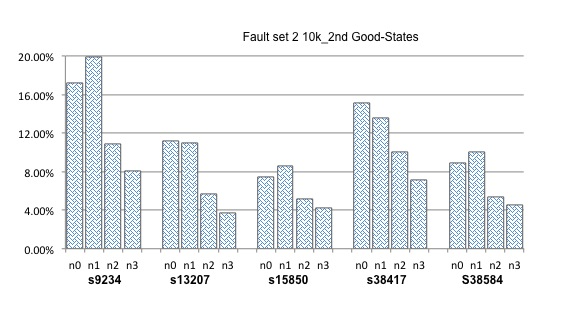
\includegraphics[scale=0.2,width = \linewidth]{../Figures/percentage_increase_set2_10k_2nd.jpg}
\end{figure}

These graphs represent the total percentage of patterns that test for non-functional defaults generated by Cell-aware ATPG out of all Stuck-at ATPG plus functional Cell-aware ATPG patterns for each of the five circuits that were tested. Here again we see that two different sets of 10\,000 good-states, as well as two different Cell-aware fault set's achieved similar results. As the n-detect redundancy increases we see a sharp decrease in the percentage of patterns that check for non-functional defects. Although even when we use n3 there remains 3~4\% of patterns testing non-functional defects this is still a dramatic decrease from the normal percentage which is around 17~18\% of all test patterns. This percentage decrease is not due to a decrease in the actual number of non-functional test patterns (as seen in figure 1), but an overall increase in the number of stuck-at ATPG patterns generated in response to the desired redundancy of the n-detect pattern generation. 


\begin{center}
\textbf{Distribution of Cell-Aware Faults Between Functional & Non-Functional for those not Detected by Stuck-At ATPG}%\par\medskip
\end{center}
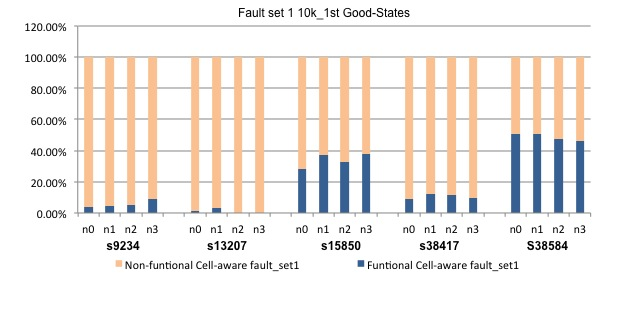
\includegraphics[scale=0.2,width = \linewidth]{../Figures/distribution_set1_10k_1st.jpg}
\end{figure}

\begin{figure}[H]
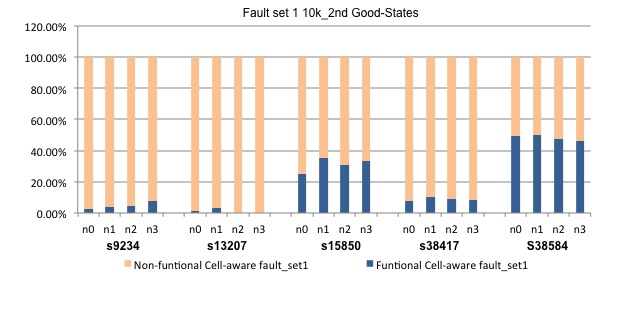
\includegraphics[scale=0.2,width = \linewidth]{../Figures/distribution_set1_10k_2nd.jpg}
\end{figure}

\begin{figure}[H]
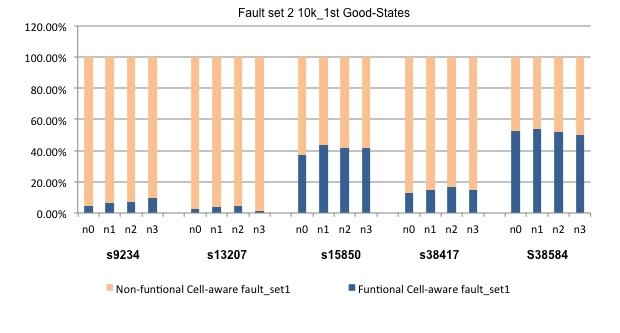
\includegraphics[scale=0.2,width = \linewidth]{../Figures/distribution_set2_10k_1st.jpg}
\end{figure}

\begin{figure}[H]
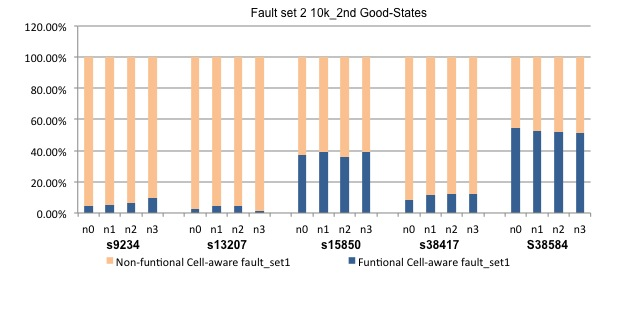
\includegraphics[scale=0.2,width = \linewidth]{../Figures/distribution_set2_10k_2nd.jpg}
\end{figure}

The above figures show the distribution of percentages of functional, and non-functional Cell-aware faults not detected by stuck-at ATPG. Once again the results were similar for all of the tested patterns and Cell-aware fault sets. Different circuits obtained different distributions based on circuits’ characters. However we can see that the non-functional Cell-aware faults that were detected accounted for a large percentage of the total Cell-aware faults for those not detected by Stack-at ATPG . In s13207 the non-functional Cell-aware faults accounted for 97-100\% of all non-detected Cell-aware faults by Stuck-at ATPG, even in s38584 non-functional Cell-aware faults accounted for 50-54\% of the total non-detected Cell-aware faults by Stuck-at ATPG. 

\begin{figure}[H]
\begin{center}
\textbf{Number of Detections for each Fault Detected by Good-State Patterns}%\par\medskip
\end{center}
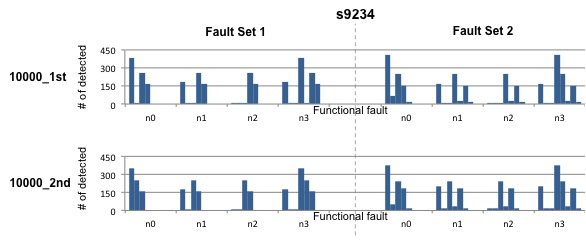
\includegraphics[scale=0.2,width = \linewidth]{../Figures/detections_s9234.jpg}
\end{figure}

\begin{figure}[H]
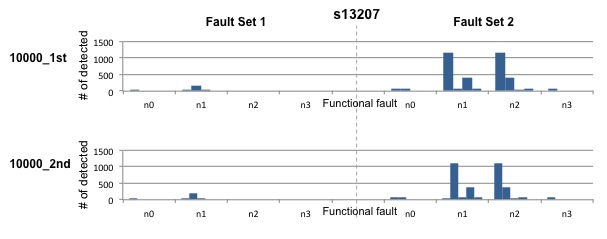
\includegraphics[scale=0.2,width = \linewidth]{../Figures/detections_s13207.jpg}
\end{figure}

\begin{figure}[H]
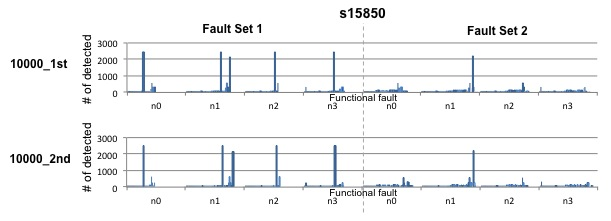
\includegraphics[scale=0.2,width = \linewidth]{../Figures/detections_s15850.jpg}
\end{figure}

\begin{figure}[H]
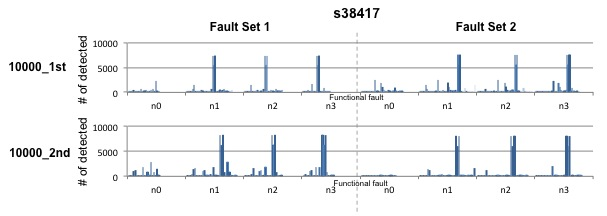
\includegraphics[scale=0.2,width = \linewidth]{../Figures/detections_s38417.jpg}
\end{figure}

\begin{figure}[H]
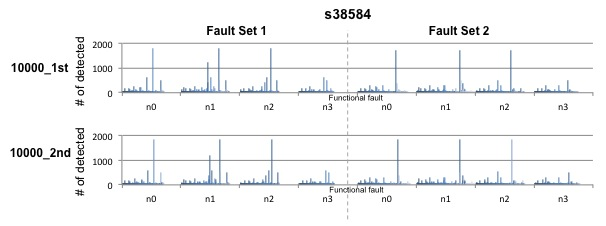
\includegraphics[scale=0.2,width = \linewidth]{../Figures/detections_s38584.jpg}
\end{figure}


Here are charts for each of the five circuits that were tested. They show the number of functional faults that were detected based on Cell-aware fault sets used and the iteration of the test. The bars above each of the n-detect numbers represent the faults detected in each set of gates: AND, NAND, NOR, and OR respectively, with 2,3, and 4 input pins each. We noticed that some faults were detected only 2 or 3 times, whereas others were detected as many as 8\,000 times. The faults that were detected many times are likely the most crucial faults. N-detect does not detect many important functional faults, even as n increases. This suggests that increasing the redundancy of the test set with n-detect is ineffective for examining these crucial functional faults.

\onecolumn
\begin{figure}
\begin{center}
\textbf{\# of Functional Faults Table}\par\medskip
\end{center}

\noindent%\hrulefill

\smallskip\noindent
\resizebox{\linewidth}{!}{%
\begin{tabular}{|c|c|c|c|c|c|c|c|c|c|c|c|c|c|c|c|c|c|c|c|c|c|}
\hline
\multicolumn{2}{|c|}{\textbf{Benchmark}} & \multicolumn{4}{|c|}{\textbf{s9234}} & \multicolumn{4}{|c|}{\textbf{s13207}} & \multicolumn{4}{|c|}{\textbf{s15850}} & \multicolumn{4}{|c|}{\textbf{s38417}} & \multicolumn{4}{|c|}{\textbf{s38584}} \\
\hline
\multicolumn{2}{|c|}{\textbf{$n$ number}} & \textbf{n0} & \textbf{n1} & \textbf{n2} & \textbf{n3} & \textbf{n0} & \textbf{n1} & \textbf{n2} & \textbf{n3} & \textbf{n0} & \textbf{n1} & \textbf{n2} & \textbf{n3} & \textbf{n0} & \textbf{n1} & \textbf{n2} & \textbf{n3} & \textbf{n0} & \textbf{n1} & \textbf{n2} & \textbf{n3} \\
\hline
\multirow{2}{*}{Fault Set 1} & 10k 1st & 4 & 5 & 5 & 7 & 1 & 3 & 0 & 0 & 26 & 41 & 31 & 37 & 26 & 38 & 31 & 23 & 153 & 177 & 142 & 128 \\ \cline{2-22} & 10k 2nd &3 &4 &4	&6 &1 &3 &0 &0 &23 &39 &29 &33 &21 &33 &24 &20 &149 &175 &141 &128	\\ 
\hline
\multirow{2}{*}{Fault Set 2} & 10k 1st & 5&7&7&8&2&4&4&1&41&53&45&47&35&46&45&36&183&216&178&160	
 \\ \cline{2-22} & 10k 2nd & 5&6&6&8&2&5&4&1&41&47&39&44&23&36&33&30&190&212&177&163
	\\ 
\hline
\end{tabular}}

\end{figure}
\twocolumn
This table shows the number of functional Cell-aware faults in each circuit, because Cell-aware faults are inserted in each of the gates we can see that the larger the circuit, the more functional Cell-aware faults are inserted.

\section{Conclusions}

\bibliography{NDetNDet}{}
\bibliographystyle{IEEEtran} 

\end{document}